\chapter{Overview of the Dual-Phase Detector Module Design}
\label{ch:fddp-ov}


%%%%%%%%%%%%%%%%%%%%%%%%%%%%%%%%%%%%%%%%%%%%%%%%%%%%%%%%%%%%%%%%%%%%
\section{Description}
\label{sec:fddp-ov-description}
This design implements a dual-phase liquid argon
time projection chamber (LArTPC) augmented with a light-readout
system. ``Dual-phase'' refers to the extraction of ionization
electrons at the interface between liquid and gas argon and their
amplification and collection in the gas phase.

The Dual Phase TPC is shown in Figure~\ref{fig:figure-label-1} with the main components.

\begin{dunefigure}[optional caption for LoF]{fig:figure-label-1}
{The DUNE dual-phase 
detector with cathode, PMTs, field cage and anode plane with chimneys.}
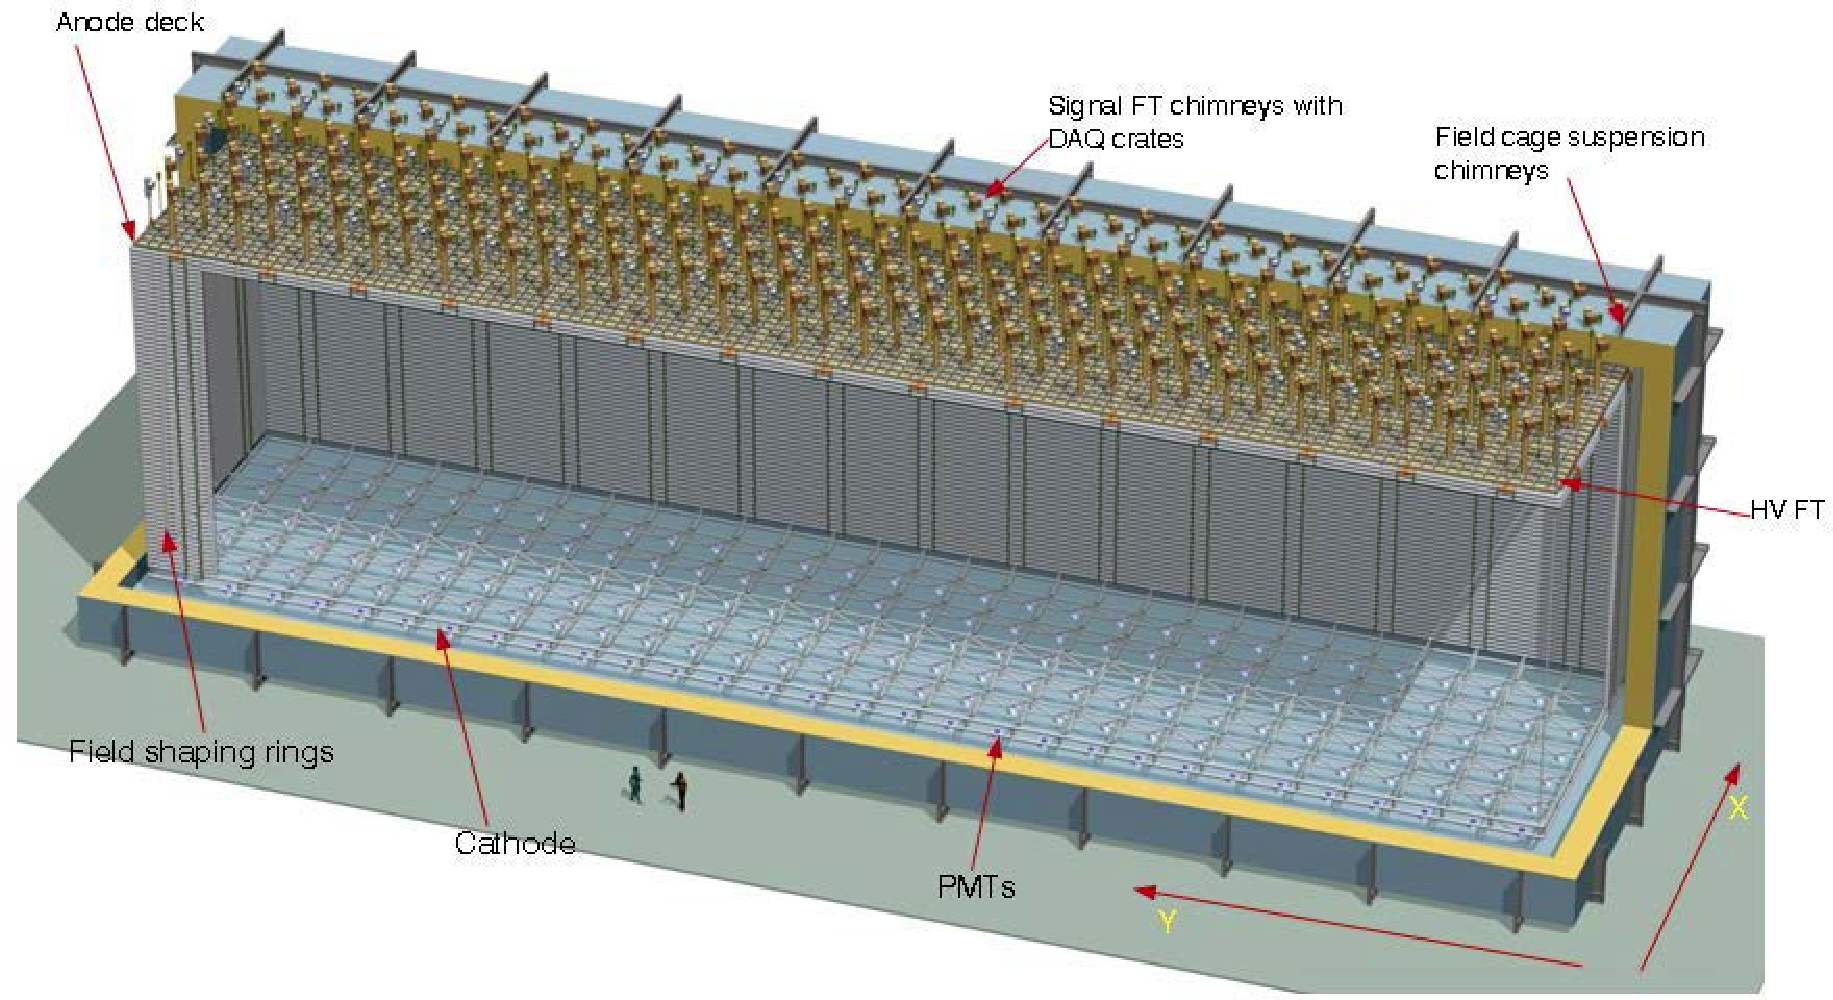
\includegraphics[width=0.8\textwidth]{DUNE-CDR-detectors-volume-optim.pdf}
\end{dunefigure}
The detector for the \ktadj{12.1} active mass module is built as a single
active volume 60~m long, 12~m wide and 12~m high, with the anode at the
top, the cathode near the bottom and an array of photon detectors (PMTs)
located at the bottom of the vessel underneath the cathode. 
The active volume (see Figure~\ref{fig:DP_det1}) is surrounded by the
field cage.

The proposed design optimally exploits the
cryostat volume of 14(w)$\times$14.1(h)$\times$62(l)~m$^3$ with an
anode active area of 12$\times$60~m$^2$ and a drift length of 12~m,
corresponding to an active mass of 12.096~kt of LAr (10.643~kt
fiducial).

The ionization electrons in the liquid phase drift  in a uniform electric field towards the anode plane at the top of the active
volume. This is made by by an array of 80 independent CRP modules, 3$\times$3~m$^2$ each.
The extraction of the electrons from the liquid to vapor phase is performed thanks to the submersed horizontal extraction grid, 
integrated in each CRP structure. A CRP unit includes 36 (0.5~m$\times$0.5~m) LEM/anode sandwiches, providing tunableamplification and charge collection on two independent views organized in strips of 3-m length and 3.125-mm pitch. There are 1920 readout channels for each CRP. Signals in each CRP unit are collected via three signal feedthrough chimneys hosting the front-end cards with the cryogenic ASIC amplifiers (640 channels/chimney) which are accessible and replaceable without contaminating the pure liquid argon volume. Each chimney is coupled to a microTCA crate ensuring the signals' digitization and 
data acquisition. These crates are connected  via optical fiber links to the DAQ back-end. The total number of readout channel 
per \ktadj{10} module is 153,600.
 
Each CRP unit is independently suspended by three stainless steel ropes. The vertical level of each CRP unit can then be automatically
adjusted with respect to the LAr level via three suspension feedthroughs, electrically operated from outside. A Slow Control feedthrough, 
one per CRP unit, is used for the signals readout for level meters and the temperature probes and to apply the HV bias on the two
sides of the LEMs and on the extraction grid. The number of components and parameters for the \ktadj{12} dual-phase LArTPC are summarized in Tables~\ref{tab:DP_params}
and~\ref{tab:DP_numbers}.

\begin{dunetable}[Sizes and dimensions for the \ktadj{12}  dual-phase LArTPC]{lll}
{DP_params}{Sizes and Dimensions for the \ktadj{12}  dual-phase  LArTPC}  Item & Value(s) &  \\ \toprowrule
Active volume width and length & W = 12~m &  L = 60~m \\ \colhline
Active volume height &  H = 12~m   &  \\ \colhline
Active volume/LAr mass & 8,640 ~m$^3$ &  12,096 metric ton \\ \colhline
Field ring vertical spacing & 200~mm  \\ \colhline
Field ring tube diameter & 140~mm \\ \colhline
Anode plane size & W = 12~m & L = 60~m \\ \colhline
CRP unit size & W = 3~m & L = 3~m  \\ \colhline
HV for vertical drift & 600~kV \\ \colhline
Resistor value & 100~M$\Omega$ \\ 
\end{dunetable}
\begin{dunetable}[Quantities of items for the \ktadj{12}  dual-phase LArTPC]{ll}{DP_numbers}{Quantities of Items for the \ktadj{12}  dual-phase  LArTPC}  Item & Number    \\ \toprowrule
Field rings & 60     \\ \colhline
CRP units & 4 $\times$ 20 = 80 \\ \colhline
LEM/Anode sadwiches per CRP unit & 36 \\ \colhline
LEM/Anode sandwiches (total) & 2,880 \\ \colhline
SFT chimneys / CRP unit & 3 \\ \colhline
SFT chimneys (total) & 240 \\ \colhline
Readout channels / SFT chimney & 640  \\ \colhline
Readout channels (total) & 153,600 \\ \colhline
Suspension FT / CRP unit & 3  \\ \colhline
Suspension FTs (total) & 240  \\ \colhline
Slow Control FT / sub-anode & 1  \\ \colhline
Slow Control FTs (total) & 80 \\ \colhline
HV feedthrough & 1  \\ \colhline
Voltage degrader resistive chains & 4 \\ \colhline
Resistors (total) & 240    \\ \colhline
PMTs (total) & 720 (1/~m$^2$) \\ 
\end{dunetable}


A number of factors make the dual-phase TPC concept as described in this chapter 
well suited to large detector sizes like the DUNE far detector.

In this design, the charge attenuation on the long drift paths is compensated by the
charge amplification in the CRPs.  This configuration also simplifies
construction by optimally exploiting the long vertical dimensions of
the cryostat, providing a large homogeneous fiducial volume 
free of embedded passive materials (effectively increasing the detector size),
reducing the number of readout channels,  and ultimately lowering costs.  
The CRPs collect the charge in a projective way,  with practically no dead region and read the signals out 
in two collection views, eliminating the need for  induction views, which 
simplifies the reconstruction of complicated topologies. The tunable high S/N provides operative margins
with respect to the noise and electron lifetime conditions and lowers the threshold on the minimal
detectable energy depositions .

The scope of a dual-phase far detector module for DUNE includes the design,
procurement, fabrication, testing, delivery, installation and
commissioning of the detector components:
\begin{itemize}
\item Charge-Readout Planes (CRP), including extraction grid, Large Electron Multiplier (LEM) and anode and readout planes;
\item Cathode, field cage and high voltage system;  
\item Electronics and data acquisition; 
\item Chimneys, isolated volumes used for electronics feedthroughs;  
\item Slow Controls; and
\item Light-readout system.
\end{itemize}

\section{Detector systems}
\label{sec:fddp-ov-systems}
\subsection{Charge Collection, Amplification and Readout}

An extraction efficiency of 100\% of the electrons from the liquid to
the gas phase is achieved with an electric field of the order of
2~kV/cm across the liquid-gas interface, applied between an 
extraction grid submersed in the liquid and charge amplification 
devices situated in the ultra-pure argon gas. 

These amplification devices, called Large Electron Multipliers (LEMs), are horizontally 
oriented 1-mm-thick printed 
circuit boards with electrodes on the top and bottom surfaces. They are drilled
through with many holes that collectively form a micro-pattern structure;  
when a 3-kV potential difference is applied across the electrodes
the ionization electrons are amplified by avalanches (Townsend multiplication) occurring in the 
pure argon gas in this micro-pattern structure due to the high electric field (30 kV/cm).

The use of avalanches to amplify the charges in the gas phase increases
the S/N ratio by at least one order of magnitude with a typical gain of 20--100, significantly
improving the event reconstruction quality. It also lowers the
threshold for small energy depositions and provides a better
resolution per volumetric pixel (voxel) compared to a single-phase
LArTPC. 

The charge is collected in a finely segmented 2D ($x$ and $y$) readout anode
plane at the top of the gas volume and fed to the front-end electronics.   

The  collection, amplification and readout components are combined in an array of 
independent (layered) modules called Charge Readout Planes (CRPs). A CRP is 
composed of several 0.5$\times$0.5-m$^2$ units, each of which is composed 
of a LEM/anode sandwich. 
These units are embedded in a mechanically reinforced frame of FR-4 and iron-nickel invar alloy. The CRP structure also integrates
 the submersed extraction grid, which is an array of $x$ and $y$ oriented stainless steel wires, 0.1~mm in diameter, with 3.125-mm
pitch. Thicknesses and possible biasing voltages for the different layers are indicated in Figure~\ref{fig:CRP_struct}.
\begin{dunefigure}[optional caption for LoF]{fig:CRP_struct}
{Thicknesses and HV values for electron extraction from liquid to gaseous Ar, their  multiplication by LEMs and their collection on the $x$ and $y$ readout anode plane. The HV values are indicated for a drift field of 0.5~kV/cm in LAr.}
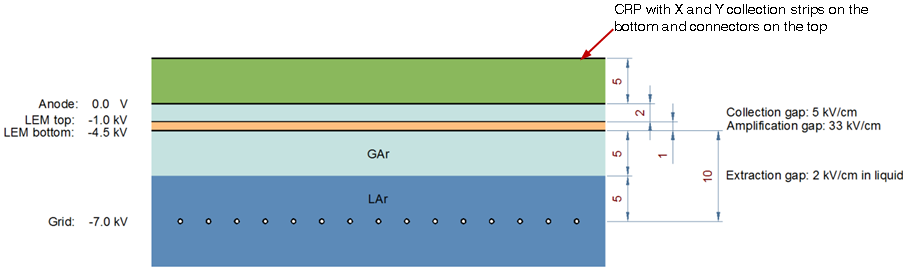
\includegraphics[width=0.8\textwidth]{CRP_gaps.png}
\end{dunefigure}

Each CRP is independently suspended with stainless-steel ropes linked to the tank top deck. This suspension system allows adjustment of the CRP distance and parallelism with respect to the LAr surface, and keeps the extraction grid immersed.

A CRP provides an adjustable charge gain (with a minimal required gain of 20) and two independent, orthogonal readout views, each with a pitch of 3.125~mm.  The LEM/anode sandwiches  in the same CRP unit are interconnected with short flat cables so that each readout channel corresponds to a total strip length of 3~m.

Combined with the time information coming from the LAr scintillation readout by
the PMT arrays ($t_0$), a CRP provides 3D track imaging with $dE/dx$ information. 
The CRPs and their components are described in Chapter~\ref{ch:fddp-CRP}.

The typical amplification achieved by this design, between 20--100, improves the S/N ratio and thus 
compensates for the charge losses that occur along the very long drift paths due to the presence of 
electronegative impurities. Therefore, despite the longer drift length, this design requires no higher 
purity of the LAr than does the reference design, around 0.1~ppb (or 100~ppt) of oxygen equivalent,
and yields a 3-ms electron lifetime. The required level of purity can be reached by starting from 
commercially available ppm-level bulk argon and filling a non-evacuated vessel\cite{WA105_TDR}.

The S/N ratio can exceed 100 for a minimum
ionizing particle (MIP) after a drift path of 12~m (given an
electron lifetime of 3~ms, a drift field of 0.5~kV/cm and a LEM gain
of 180). With the same drift field, the same electron-lifetime conditions and a
LEM gain of 25, the S/N is larger than 50:1 for tracks up to 6~m from
the anode; it reaches 14:1 for MIP tracks that are 12~m from the
anode.


\subsection{Electronics and ``Chimneys''}
 
The electrical signals from the collected charges
are passed to the outside of the tank via a set of dedicated signal
feedthrough ``chimneys'' (insulated volumes filled with nitrogen
that pass through the top layer of insulation). 
The cryogenic front-end (FE) electronics cards, housed at the bottom of the
chimneys, are based on analog preamplifiers implemented in CMOS ASIC circuits for high integration and large-scale
affordable production. Within the chimneys, the cards are actively cooled to a temperature of about 110 K and
isolated with respect to the LAr vessel by a cold feedthrough.  This
feedthrough is connected to the CRP via short flat cables of (0.5~m length) in order to minimize the
input capacitance to the preamplifiers. Each chimney collects 640 readout channels.

The chimney design allows access to and replacement of the FE from the
outside without contaminating the LAr volume. The digital electronics
and DAQ system are completely outside the cryostat and are housed in
microTCA racks mounted on each signal feedthrough chimney. 

Other feedthroughs are planned for the cathode HV connection, the
CRPs' suspension and level adjustment, the high voltage and signal
readout of the PMTs, and the monitoring instrumentation (level meters,
temperature probes, strain gauges, etc.).

\subsection{Cathode, Field Cage and HV System}
\label{v4:fd-alt-ov:cathode}

The drift field (E ${\simeq}$ 0.5~kV/cm) inside the fully
active LAr volume is produced by applying high voltage to the cathode
plane at the bottom of the cryostat and is kept uniform by the field cage, a stack
of 60 equally spaced field-shaping electrodes,  
polarized at linearly decreasing voltage from the cathode 
voltage to almost ground potential, reached at the level of the charged readout plane.
The electrodes are rectangles made of stainless-steel tubes  (diameter 140~mm,  vertical pitch 200~mm)
with rounded corners, running horizontally (and stacked vertically) around the
active volume.


The field cage is held in place by mechanical structures hung from the
top deck of the vessel that also provide insulation.  The cathode
structure, constructed of a reinforced frame to 
guarantee its planarity, is suspended from the field cage and hangs near the 
bottom of the cryostat. It is a segmented structure of tubes of different sizes 
arranged in a grid to minimize weight, limit sagging and avoid high electric field
regions in its proximity.  The segmented structure allows scintillation light to pass
through and be detected by uniform arrays of photomultipliers (PMTs) mounted
1~m below it at the bottom of the tank.
